\chapter{Design Specifications}\label{chap:specifications}


\section{Requirements}\label{requirements}
Based on the design considerations and limitations explained earlier in this report, a list of requirements shall be developed.
%
\begin{enumerate}
\item \textbf{The Cubli should be able to balance starting from an unstable equilibrium position and a null velocity.}
  \begin{itemize}
  \item[] Considering only naturally occurring perturbations, the Cubli needs to be able to regulate its position by itself, around \si{0\ rad}, without falling directly.
  \end{itemize}

\item \textbf{The prototype should be able to balance around \si{0\ \rad} regardless of the level of the baseplate, using internally mounted sensors.}  
  \begin{itemize}
  \item[] This ensures that the 2D design of the Cubli can keep its upright position independently from its base plate and therefore, can be more easily translated to a 3D model.
  \end{itemize}
%  
%\item \textbf{The Cubli should be balancing during X \si{s}.}\fxnote{A number should be determined for X.}
%  	\begin{itemize}
%  		\item[] The amount of time the system stands should be measured from the moment the controller starts acting on the plant, with initial conditions an unstable equilibrium position (aproximately \si{0\ rad \cdot s^{-1}}) with a null velocity of the wheel and the frame. The timer should be stopped as soon as the Cubli falls outside of the active region of the controller.
%  	\end{itemize}
%  	
%\item \textbf{The implemented controller should keep the Cubli within X \si{rad \cdot s^{-1}}.}\fxnote{A number has to be determined for Xand more arguments should be given.}
\end{enumerate}
%
From these established requirements, a controller allowing the Cubli to stabilize in an upright position is to be designed and implemented.

\section{Further Capabilities Analysis}\label{title}
Moreover, a further investigation on the behavior of the controlled system is to be done in order to determine the capabilities of the final prototype. This includes:
\begin{enumerate}
\item \textbf{Duration of the stable operation}
	\begin{itemize}
	\item[] How long can the Cubli be in equilibrium until the controller in not able to balance it.
	\end{itemize}

	\item \textbf{Maximum recovery angle}
	\begin{itemize}
		\item[] Once the Cubli is balance, its position is forced to change to different angles and the capability of tit to go back to the equilibrium position is checked. 
	\end{itemize}
	
	\item \textbf{Maximum catching angle with no initial velocity of the wheel}
	\begin{itemize}
		\item[] The maximum starting angle the system can have and still be able to balance is to be tested.\\
		However, there exists a limitation which is given by the maximum current that the motor can provide which conditions the maximum catching angle. As can be seen in \figref{limitationTorque}, if the initial angle is different from 0 rad both the mass of the frame ans the mass of the wheel exert an initial torque to the system. This must be overcame by the motor to avoid the Cubli to fall.
		%
		\begin{figure}[H] 
			\centering
			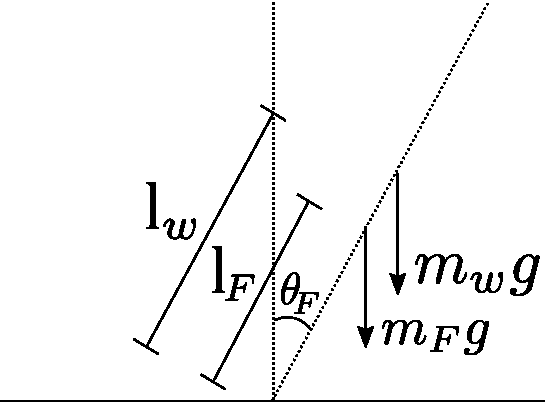
\includegraphics[scale=0.65]{figures/limitationTorque}
			\caption{Force acting on the system that create an initial torque}
			\label{limitationTorque}
		\end{figure}
		
		The minimum torque that the motor must apply is give by \eqref{minTorque}.
		%
		\begin{flalign}
		\eq{T} { (m_F \cdot l_F + m_w \cdot l_w) \cdot g \cdot sin(\theta_F)} \unit{N\cdot m}
		\label{minTorque}
		\end{flalign}
		
		Since the torque is restricted by the characteristics of the motor and the control board, the maximum initial angle is derived in \eqref{maxAngle}.
		%
		\begin{flalign}
		\eq{\theta_F} { asin\left(\frac{T}{(m_F \cdot l_F + m_w \cdot l_w) \cdot g}\right)} \unit{N\cdot m}
		\label{maxAngle}
		\end{flalign}
		%
		Substituding the values of the maximum torque (see section \ref{sec:Motor}) and the parameters of the Cubli (see section \ref{sec:Param}) the maximum starting angle is \si{0,2024\ rad}.

	\end{itemize}
	
\end{enumerate}